%% This is the ctufit-thesis example file. It is used to produce theses
%% for submission to Czech Technical University, Faculty of Information Technology.
%%
%% Get the newest version from
%% https://gitlab.fit.cvut.cz/theses-templates/FITthesis-LaTeX
%%
%%
%% Copyright 2021, Eliska Sestakova and Ondrej Guth
%%
%% This work may be distributed and/or modified under the
%% conditions of the LaTeX Project Public Licenese, either version 1.3
%% of this license or (at your option) any later version.
%% The latest version of this license is in
%%  https://www.latex-project.org/lppl.txt
%% and version 1.3 or later is part of all distributions of LaTeX
%% version 2005/12/01 or later.
%%
%% This work has the LPPL maintenance status `maintained'.
%%
%% The current maintainer of this work is Ondrej Guth.
%% Contact ondrej.guth@fit.cvut.cz for bug reports.
%% Alternatively, submit bug reports into the tracker at
%% https://gitlab.fit.cvut.cz/theses-templates/FITthesis-LaTeX/issues
%%
%%

%%%%%%%%%%%%%%%%%%%%%%%%%%%%%%%%%%%%%%%%%
% CLASS OPTIONS
% language: czech/english/slovak
% thesis type: bachelor/master/dissertation
%%%%%%%%%%%%%%%%%%%%%%%%%%%%%%%%%%%%%%%%%
\documentclass[czech,bachelor,unicode]{ctufit-thesis}

%%%%%%%%%%%%%%%%%%%%%%%%%%%%%%%%%%
% FILL IN THIS INFORMATION
%%%%%%%%%%%%%%%%%%%%%%%%%%%%%%%%%%
\ctufittitle{Systém pro~sportovní kluby} % replace with the title of your thesis
\ctufitauthorfull{Lukáš Paukert} % replace with your full name (first name(s) and then family name(s) / surname(s)) including academic degrees
\ctufitauthorsurnames{Paukert} % replace with your surname(s) / family name(s)
\ctufitauthorgivennames{Lukáš} % replace with your first name(s) / given name(s)
\ctufitsupervisor{Ing.\,Filip Glazar} % replace with name of your supervisor/advisor (include academic degrees)
\ctufitdepartment{Katedra softwarového inženýrství} % replace with the department of your defence
\ctufityear{2022} % replace with the year of your defence
\ctufitdeclarationplace{Praze} % replace with the place where you sign the declaration
\ctufitdeclarationdate{\today} % replace with the date of signature of the declaration
\ctufitabstractCZE{Fill in abstract of this thesis in Czech language. Class aptent taciti sociosqu ad litora torquent per conubia nostra, per inceptos hymenaeos. Cras pede libero, dapibus nec, pretium sit amet, tempor quis. Sed vel lectus. Donec odio tempus molestie, porttitor ut, iaculis quis, sem. Suspendisse sagittis ultrices augue.}
\ctufitabstractENG{Fill in abstract of this thesis in English language. Class aptent taciti sociosqu ad litora torquent per conubia nostra, per inceptos hymenaeos. Cras pede libero, dapibus nec, pretium sit amet, tempor quis. Sed vel lectus. Donec odio tempus molestie, porttitor ut, iaculis quis, sem. Suspendisse sagittis ultrices augue.}
\ctufitkeywordsCZE{enter, commma, separated, list, of, keywords, in, CZECH}
\ctufitkeywordsENG{enter, commma, separated, list, of, keywords, in, ENGLISH}
%%%%%%%%%%%%%%%%%%%%%%%%%%%%%%%%%%
% END FILL IN
%%%%%%%%%%%%%%%%%%%%%%%%%%%%%%%%%%

%%%%%%%%%%%%%%%%%%%%%%%%%%%%%%%%%%
% CUSTOMIZATION of this template
% Skip this part or alter it if you know what you are doing.
%%%%%%%%%%%%%%%%%%%%%%%%%%%%%%%%%%

\RequirePackage{iftex}[2020/03/06]
\iftutex % XeLaTeX and LuaLaTeX
    \RequirePackage{ellipsis}[2020/05/22] %ellipsis workaround for XeLaTeX
\else
    \RequirePackage[utf8]{inputenc}[2018/08/11] %this file encoding
    \RequirePackage{lmodern}[2009/10/30] % vector flavor of Computer Modern font
\fi

% hyperlinks
\RequirePackage[pdfpagelayout=TwoPageRight,colorlinks=false,allcolors=decoration,pdfborder={0 0 0.1}]{hyperref}[2020-05-15]

% uncomment the following to hide all hyperlinks
% \RequirePackage[pdfpagelayout=TwoPageRight,hidelinks]{hyperref}[2020-05-15]

\RequirePackage{pdfpages}[2020/01/28]

\setcounter{secnumdepth}{4} % numbering sections; 4: subsubsection

% Added / customized
\usepackage{bbding} % checkmarks

\usepackage{enumitem} % lists
% Specially customized item for enumerate
% Source: https://github.com/tenhobi/bachelors-thesis/blob/master/macros/my-item.tex
%
% [1]
% Description

\newcommand{\myItem}[1]{\item{\textbf{#1}}\newline}

% Environment for numbered lists on second level

\newenvironment{enumerateNumbers}
	{\begin{enumerate}[label=\textcolor{decoration}{\textbf{\arabic*.}}]} 
	{\end{enumerate}}


\usepackage{tabularx} % tables
% New column types used with tabularx package

\newcolumntype{L}{>{\raggedright\arraybackslash}X}
\newcolumntype{R}{>{\raggedleft\arraybackslash}X}
\newcolumntype{C}{>{\centering\arraybackslash}X}


\usepackage{pdflscape}

%%%%%%%%%%%%%%%%%%%%%%%%%%%%%%%%%%
% CUSTOMIZATION of this template END
%%%%%%%%%%%%%%%%%%%%%%%%%%%%%%%%%%


%%%%%%%%%%%%%%%%%%%%%%
% DEMO CONTENTS SETTINGS
% You may choose to modify this part.
%%%%%%%%%%%%%%%%%%%%%%
\usepackage{dirtree}
\usepackage{lipsum,tikz}
\usepackage{csquotes}
\usepackage[style=iso-numeric]{biblatex}
\addbibresource{parts/bib-database.bib}
\usepackage{listings} % typesetting of sources
% \usepackage{minted} % typesetting of sources

%theorems, definitions, etc.
\theoremstyle{plain}
\newtheorem{theorem}{Věta}
\newtheorem{lemma}[theorem]{Tvrzení}
\newtheorem{corollary}[theorem]{Důsledek}
\newtheorem{proposition}[theorem]{Návrh}
\newtheorem{definition}[theorem]{Definice}
\theoremstyle{definition}
\newtheorem{example}[theorem]{Příklad}
\theoremstyle{remark}
\newtheorem{note}[theorem]{Poznámka}
\newtheorem*{note*}{Poznámka}
\newtheorem{remark}[theorem]{Pozorování}
\newtheorem*{remark*}{Pozorování}
\numberwithin{theorem}{chapter}
%theorems, definitions, etc. END
%%%%%%%%%%%%%%%%%%%%%%
% DEMO CONTENTS SETTINGS END
%%%%%%%%%%%%%%%%%%%%%%

\begin{document} 
\frontmatter\frontmatterinit % do not remove these two commands

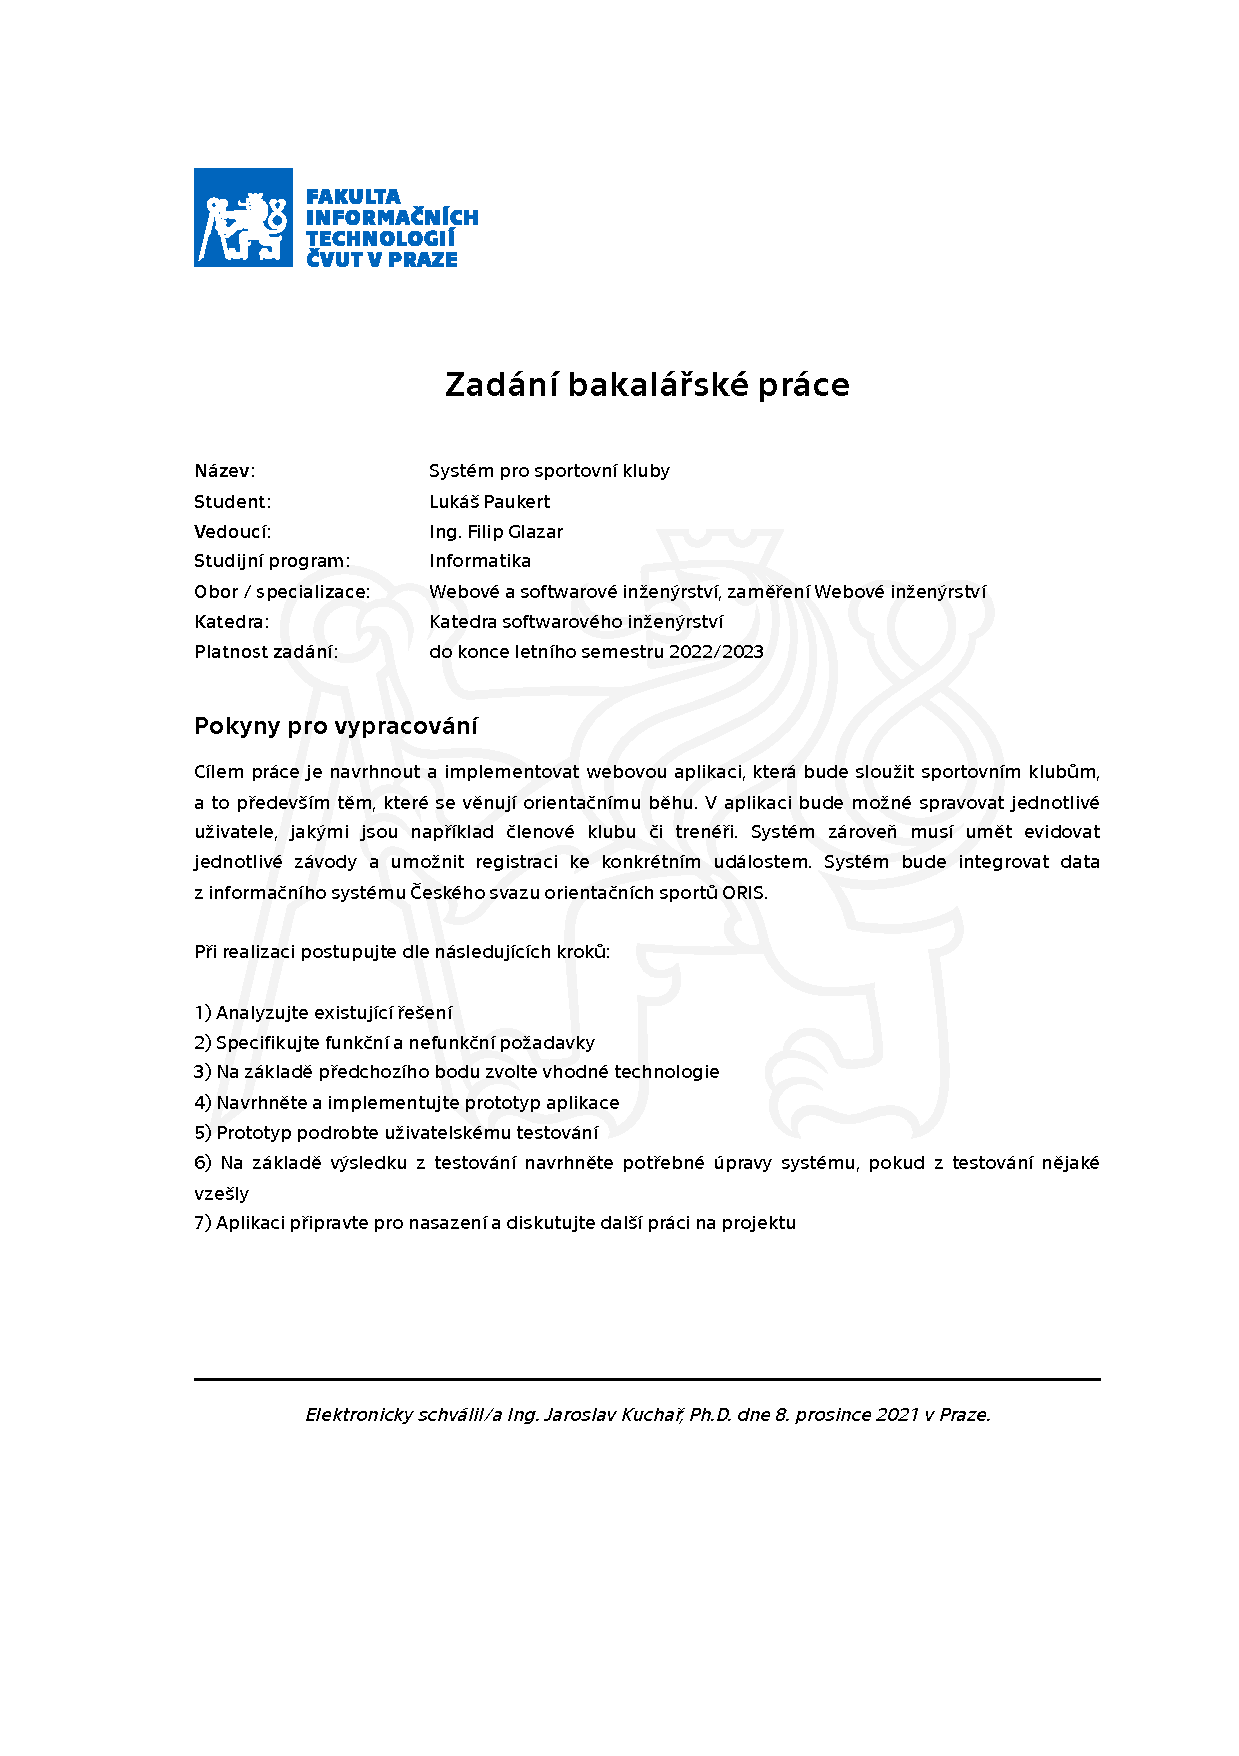
\includepdf{assignment-include.pdf} % replace that file with your thesis assignment provided by study office

\thispagestyle{empty}\cleardoublepage\maketitle % do not remove these three commands

\imprintpage % do not remove this command

\tableofcontents % do not remove this command
%%%%%%%%%%%%%%%%%%%%%%
% list of other contents: figures, tables, code listings, algorithms, etc.
% add/remove commands accordingly
%%%%%%%%%%%%%%%%%%%%%%
\listoffigures % list of figures
\begingroup
\let\clearpage\relax
\listoftables % list of tables
\lstlistoflistings % list of source code listings generated by the listings package
% \listoflistings % list of source code listings generated by the minted package
\endgroup
%%%%%%%%%%%%%%%%%%%%%%
% list of other contents END
%%%%%%%%%%%%%%%%%%%%%%

%%%%%%%%%%%%%%%%%%%
% ACKNOWLEDGMENT
% FILL IN / MODIFY
% This is a place to thank people for helping you. It is common to thank your supervisor.
%%%%%%%%%%%%%%%%%%%
\begin{acknowledgmentpage}
	Chtěl bych poděkovat především sit amet, consectetuer adipiscing elit. Curabitur sagittis hendrerit ante. Class aptent taciti sociosqu ad litora torquent per conubia nostra, per inceptos hymenaeos. Cras pede libero, dapibus nec, pretium sit amet, tempor quis. Sed vel lectus. Donec odio tempus molestie, porttitor ut, iaculis quis, sem. Suspendisse sagittis ultrices augue.
\end{acknowledgmentpage} 
%%%%%%%%%%%%%%%%%%%
% ACKNOWLEDGMENT END
%%%%%%%%%%%%%%%%%%%


%%%%%%%%%%%%%%%%%%%
% DECLARATION
% FILL IN / MODIFY
%%%%%%%%%%%%%%%%%%%
% INSTRUCTIONS
% ENG: choose one of approved texts of the declaration. DO NOT CREATE YOUR OWN. Find the approved texts at https://courses.fit.cvut.cz/SFE/download/index.html#_documents (document Declaration for FT in English)
% CZE/SLO: Vyberte jedno z fakultou schvalenych prohlaseni. NEVKLADEJTE VLASTNI TEXT. Schvalena prohlaseni najdete zde: https://courses.fit.cvut.cz/SZZ/dokumenty/index.html#_dokumenty (prohlášení do ZP)
\begin{declarationpage}
FILL IN ACCORDING TO THE INSTRUCTIONS. VYPLŇTE V SOULADU S POKYNY. Lorem ipsum dolor sit amet, consectetuer adipiscing elit. Curabitur sagittis hendrerit ante. Class aptent taciti sociosqu ad litora torquent per conubia nostra, per inceptos hymenaeos. Cras pede libero, dapibus nec, pretium sit amet, tempor quis. Sed vel lectus. Donec odio tempus molestie, porttitor ut, iaculis quis, sem. Suspendisse sagittis ultrices augue. Donec ipsum massa, ullamcorper in, auctor et, scelerisque sed, est. In sem justo, commodo ut, suscipit at, pharetra vitae, orci. Pellentesque pretium lectus id turpis.

Lorem ipsum dolor sit amet, consectetuer adipiscing elit. Curabitur sagittis hendrerit ante. Class aptent taciti sociosqu ad litora torquent per conubia nostra, per inceptos hymenaeos. Cras pede libero, dapibus nec, pretium sit amet, tempor quis. Sed vel lectus. Donec odio tempus molestie, porttitor ut, iaculis quis, sem. Suspendisse sagittis ultrices augue. Donec ipsum massa, ullamcorper in, auctor et, scelerisque sed, est. In sem justo, commodo ut, suscipit at, pharetra vitae, orci. Pellentesque pretium lectus id turpis.
\end{declarationpage}
%%%%%%%%%%%%%%%%%%%
% DECLARATION END
%%%%%%%%%%%%%%%%%%%

\printabstractpage % do not remove this command

%%%%%%%%%%%%%%%%%%%
% SUMMARY
% FILL IN / MODIFY
% OR REMOVE ENTIRELY (upon agreement with your supervisor)
% (appropriate to remove in most theses)
%%%%%%%%%%%%%%%%%%%
\begin{summarypage}
\section*{Summary section}

\lipsum[1][1-8]

\section*{Summary section}

\lipsum[2][1-6]

\section*{Summary section}

\lipsum[3]

\section*{Summary section}

\lipsum[2]

\section*{Summary section}

\lipsum[1][1-8] Lorem lorem lorem.
\end{summarypage}
%%%%%%%%%%%%%%%%%%%
% SUMMARY END
%%%%%%%%%%%%%%%%%%%

%%%%%%%%%%%%%%%%%%%
% ABBREVIATIONS
% FILL IN / MODIFY
% OR REMOVE ENTIRELY
% List the abbreviations in lexicography order.
%%%%%%%%%%%%%%%%%%%
\chapter{Seznam zkratek}
	
\begin{tabular}{rl}
API & rozhraní pro programování aplikací\\
    & (z anglického Application Programming Interface)\\
GDPR & Obecné nařízení o ochraně osobních údajů\\
	 & (z anglického General Data Protection Regulation)\\
IS ORIS & Informační systém Českého svazu orientačních sportů\\
JSON & JavaScriptový objektový zápis\\
     & (z anglického JavaScript Object Notation)\\
UI & uživatelské rozhraní (z anglického User Interface)
\end{tabular}
%%%%%%%%%%%%%%%%%%%
% ABBREVIATIONS END
%%%%%%%%%%%%%%%%%%%

\mainmatter\mainmatterinit % do not remove these two commands

%%%%%%%%%%%%%%%%%%%
% THE THESIS
% MODIFY ANYTHING BELOW THIS LINE
%%%%%%%%%%%%%%%%%%%

\chapter{Úvod}
\section{Motivace}
Již od~mala jsem rád věnoval svůj volný čas různým sportovním aktivitám. Chvilku jsem navštěvoval plavecký kroužek, poté jsem hrál fotbal, tenis a~jednoho dne jsem se díky kamarádovi dostal i~k~orientačnímu běhu, u~kterého jsem nakonec zůstal. Každý týden jsme mívali pravidelné tréninky a~o~víkendech jsme se účastnili závodů ve východočeské oblasti.

Na~závody jsme se ze~začátku přihlašovali vedoucímu našeho klubu pomocí e-mailu, zprávou na~Facebooku nebo~pomocí jakéhokoliv jiného komunikačního kanálu. S~rozšiřující se členskou základnou klubu však tento způsob přihlašování přestával být udržitelný, a~proto vzniklo klubové fórum, které mělo způsob přihlašování sjednotit. Kvůli kompexnosti nasazeného řešení však nebylo přihlašování na~závody pro~členy klubu tak jednoduché a~přímočaré, jak bychom si přáli. Z~tohoto důvodu jsem v~druhé polovině roku 2016 vytvořil novou webovou aplikaci, která od~roku 2017 nahradila používané diskuzní fórum.

Samotná webová aplikace bude podrobněji přestavena v~sekci \ref{section:kuoris}, avšak jelikož se jednalo o~jeden z~mých prvních programátorských projektů, tak nyní i~sám vidím, že nebyl navržen ani~naprogramován nejlépe. V~rámci své bakalářské práce bych chtěl proto celou aplikaci přepracovat a~při~této příležitosti přidat i~nové funkcionality, které zjednoduší procesy spojené s~přihlašováním na~závody a~tréninky.

\section{Cíle práce}
V~rámci své bakalářské práce vytvořím novou webovou aplikaci, která bude v~porovnání se současným řešením uživatelsky přívětivější a~která bude obsahovat i~nové funkcionality, jež výrazně zjednoduší procesy spojené s~přihlašováním na~tréninky a~závody. Aplikace musí umožňovat správu uživatelů a~událostí. Na~jednotlivé události se bude možné registrovat a~přihlášky bude následně možné odeslat do~informačního systému Českého svazu orientačních sportů ORIS.

Samotné implementaci prototypu bude předcházet analýza, která bude mimo jiné zahrnovat popis již existujících řešení a~specifikaci funkčních a~nefunkčních požadavků. Následovat bude návrh aplikace a~výběr vhodných technologií. Po~implementaci bude systém podroben uživatelskému testování a~na základě výsledků budou navrženy potřebné úpravy. V neposlední řadě bude aplikace připravena pro~nasazení místo aktuálně využívaného systému.


\chapter{Analýza}
\section{Existující řešení}
Následující podkapitola je věnována již existujícím informačním systémům, které by měly usnadnit sportovním klubům a~skupinám administrativní činnost. V~současné době jich na~trhu existuje již~poměrně velké množství, a~proto se zaměřím pouze na~ty, které mi přišly nejrozšířenější nebo~nějakým způsobem zajímavé. V~následujících sekcích budou přiblížena dvě řešení z~komerční sféry, jeden bezplatný systém a~také bude podrobněji představena aplikace, která je v~současné době využívána klubem KOB~Ústí nad~Orlicí.

Několik systémů, které mají řešit podobné problémy, vzniklo v~minulosti i~v~rámci závěrečných prací na~různých českých univerzitách. Pro~kompletnost mohu například zmínit práce \cite{fimuni2021, fitcvut2016, fisvse2013}, avšak jejich obsah zde nebudu detailněji rozebírat.

\subsection{KUOris}
\label{section:kuoris}
Klub orientačního běhu~Ústí nad~Orlicí nyní využívá pro~přihlašování na~závody webovou aplikaci KUOris. Tento systém vznikl v~roce 2016 jako nástupce řešení, které bylo založené na~open source systému phpBB, jenž je nejčastěji využíván pro~tvorbu diskuzního fóra \cite{phpbb}. V~průběhu let byl drobně upravován, avšak z~důvodu špatného návrhu není možné do~systému KUOris jednoduše přidávat nové funkcionality.

Systém v aktuálním stavu podporuje přidávání a~následné spravování událostí. Při~vytváření události se členům klubu, kteří si tuto funkcionalitu povolili, zasílá informační e-mail se základními informacemi o~dané akci. Na~jednotlivé události se členové klubu mohou přihlašovat a~mohou k~nim psát komentáře.

Mezi~největší nedostatky aplikace KUOris se řadí zastaralé uživatelské rozhraní a~chybějící automatizace. V~dnešní době, kdy na~web přistupuje více lidí z~mobilních zařízení než~z~počítačů~\cite{deviceusage}, by mělo být uživatelské rozhraní jistě responzivní. Další již zmíněný nedostatek spatřuji u nevyužité možnosti automatizace. IS~ORIS nabízí API, jež je detailněji popsané v sekci \ref{implementation:oris-api}, pro~získávání informací o~závodech a~i~pro~přihlašování na~jednotlivé akce. V současném systému této možnosti není využíváno a~všechny úkony tedy musí administrátor provádět ručně.

\begin{description}
	\item[Nevýhody:] složitá rozšiřitelnost, neresponzivní UI, absence propojení s~IS ORIS
\end{description}

\subsection{KIS~–~Klubový Informační Systém}
KIS je komplexní klubový informační systém, který je díky svým pokročilým funkcionalitám využíván i~největšími sportovními subjekty v~České republice. Mezi uživatele systému se totiž například řadí Český svaz ledního hokeje, Fotbalová asociace České republiky, Český olympijský výbor a~další velké fotbalové a~hokejové kluby. \cite{esports, ceskyhokej}

Mezi klíčové funkčnosti systému se řadí podpora pro~pořádání klubových akcí, správa plateb, evidence dokumentů, zobrazování statistik, kalendář a~mnoho dalších funkcí. K~systému je možné přistupovat i~přes~mobilní aplikaci, která je dostupná pro~zařízení s~operačním systém iOS a~Android. Jedná se o~komerční systém, dle ceníku se cena skládá z~jednorázového počátečního poplatku 9~900~Kč bez~DPH a~následného měsíčního poplatku 300~Kč bez~DPH za~technickou správu. \cite{esports}

\begin{description}
	\item[Výhody:] komplexní klubový systém s~pokročilými funkcemi a~mobilní aplikací
	\item[Nevýhody:] nákladnost (jednorázový a~následné měsíční poplatky), absence propojení s~IS ORIS
\end{description}

\subsection{Sportes~–~Český sportovní evidenční systém}
Jedná se o~další komplexní systém pro~sportovní kluby, ke~kterému je opět možné přistupovat jak z~webového prohlížeče, tak i~z~mobilní aplikace. Obsahuje podobné funkcionality jako systém KIS, tj.~správu událostí, evidenci členské základny, docházky a~plateb. Pro~menší sportovní kluby však pravděpodobně bude překážkou pro~jeho využívání uvedená cena, neboť za~variantu pro~maximálně 100~členů je stanovena na~12~000~Kč bez~DPH ročně. \cite{sportes}

\begin{description}
	\item[Výhody:] systém pro kompletní správu sportovního klubu s vlastní mobilní aplikací
	\item[Nevýhody:] nákladnost (12~000~Kč za~rok bez~DPH), absence propojení s~IS ORIS
\end{description}

\subsection{Týmuj}
Týmuj je online služba, která byla do~ostrého provozu spuštěna v~květnu roku 2008. Od~té doby v ní bylo vytvořeno přes~30~000~týmů a~svůj účet si vytvořilo přes~250~000~sportovců. Služba Týmuj je od~svého vzniku neustále vylepšována a~v~roce 2017 byly spuštěny i~mobilní aplikace pro~operační systémy iOS a~Android.

Týmuj umožňuje vytvářet a~spravovat události, evidovat docházku u~jednotlivých událostí, posílat zprávy do~týmového chatu a~k~jednotlivým akcím, evidenci týmových plateb, sdílení fotografií a~mnoho dalších věcí. V~rámci týmu mají jednotliví členové jednu ze~tří rolí (majitel, správce nebo~hráč) a~na~základě přidělené role mají odpovídající práva.

Popularitu tohoto online nástroje dokazuje fakt, že jen za~poslední rok bylo přes~Týmuj zorganizováno přes~300~000~událostí. Takový počet akcí bude jistě z~nemalé části způsoben tím, že využívání Týmuj není zpoplatněno a~že~taktéž neexistuje omezení na~maximální počet členů týmu. \cite{tymuj}

\begin{description}
	\item[Výhody:] užívání není zpoplatněno, obsahuje mnoho funkcí, existuje webová i mobilní aplikace
	\item[Nevýhody:] absence propojení s~IS ORIS
\end{description}
\newpage

\section{Funkční požadavky}
Funkční požadavky popisují požadované funkcionality systému. Mohou například specifikovat, jakým způsobem bude uživatel moci pracovat se systémem, jaké procesy by měl systém podporovat a~jaké budou vstupy a~výstupy těchto procesů. \cite{requirements}

\begin{enumerate}[label=\textcolor{decoration}{\textbf{F\arabic*}}, leftmargin=6mm]
	\myItem{evidence a~správa uživatelů}
	Systém bude umožňovat registraci nových uživatelů, neregistrovaný uživatel nemá přístup do~systému. Při~registraci bude nutno zadat minimálně registrační číslo, e-mailovou adresu, heslo a~jméno a~příjmení člena klubu. Právě pomocí registračního čísla a~zadaného hesla bude následně uživatel přistupovat do~systému.

	Kromě těchto základních údajů bude mít administrátor možnost uživateli nastavovat a~upravovat stav osobního konta, typ členství (aktivní nebo~pasivní) a~roli (viz~sekce \ref{section:role}). Uživatele musí být možno anonymizovat kvůli GDPR.

	\myItem{evidence a~správa závodů a~tréninků\label{f:events}}
	Dále systém bude umožňovat evidenci a~správu tréninků a~závodů (událostí). Konkrétně je potřeba mít možnost u~každé události evidovat:
	\begin{itemize}
		\item název
		\item typ události (trénink nebo~závod)
		\item datum a~čas události (kdy událost začíná)
		\item místo konání
		\item pořadatel
		\item datum a~čas uzávěrky přihlášek
		\item disciplínu
		\item vypsané kategorie
		\item další informace
		\item v~případě závodu bude možné dále evidovat:
		\begin{itemize}
			\item typ závodu
			\item webovou stránku
		\end{itemize}
		\item u~tréninku bude možné oproti závodu naopak evidovat maximální kapacitu
	\end{itemize}

	Samotné zadání události do~systému bude umožněno ručním vyplněním všech požadovaných údajů nebo~automatickým importem z~informačního systému Českého svazu orientačních sportů pomocí unikátního identifikátoru závodu.

	Na~hlavní stránce systému by se měly zobrazovat závody a tréninky s~nejbližší uzávěrkou přihlášek. V~zadaných trénincích a~závodech bude možné vyhledávat a~filtrovat a~zadanou událost musí být možno zrušit bez~odstraňování ze~systému. Taková událost bude následně od~nezrušených událostí vizuálně odlišena a~nebude možné se na~ni dále přihlašovat.

	\myItem{přihlašování na~závody a~tréninky}
	Na~událost evidovanou v~systému se mohou registrovaní uživatelé přihlásit, pokud dosud neproběhla uzávěrka přihlášek. Při~přihlášení si uživatelé musí navíc vybrat jednu z~nabízených kategorií, do~které se chtějí přihlásit, a~mohou volitelně sdělit, zdali mají možnost jet vlastním autem a~svést s~sebou i~další členy klubu. Svou účast mohou uživatelé do~konce uzávěrky přihlášek také odřeknout.

	\myItem{synchronizace přihlášek}
	Po~skončení termínu přihlášek bude mít trenér možnost odeslat všechny evidované přihlášky do~IS~ORIS přes~jeho API. Tato možnost bude ze~zřejmých důvodů dostupná pouze pro~závody, které jsou v~IS~ORIS evidované.

	\myItem{e-mailová upozornění --- TODO: asi odebrat}
	Systém bude umožňovat při~přidávání události odeslat informační e-mail se základními informacemi o~dané události. E-mail bude odeslán pouze těm registrovaným uživatelům, kteří si ve~svém nastavení povolili zasílání e-mailových upozornění.

	\myItem{oznámení}
	Trenéři a~administrátoři systému budou mít možnost vytvořit oznámení, která se budou zobrazovat na~hlavní stránce systému.

	\myItem{komentáře}
	Komentáře mohou psát registrovaní uživatelé ke~všem tréninkům a~závodům. Nejnovější komentáře by se měly zobrazovat (včetně informace kam byly napsány) na~hlavní stránce systému.
\end{enumerate}

\subsection{Role}
\label{section:role}
Každému uživateli bude náležet právě jedna z~následujících uživatelských rolí:
\begin{itemize}
	\item registrovaný uživatel
	\begin{itemize}
		\item základní uživatelská role, která nemá žádná speciální oprávnění
		\item výčet akcí, které může registrovaný uživatel vykonávat:
		\begin{itemize}
			\item přihlašovat a~odhlašovat se z~tréninků a~závodů
			\item psát komentáře k~jednotlivým tréninkům a~závodům a~následně je i~upravovat
			\item měnit svou e-mailovou adresu a~heslo pro~přihlášení do~systému
			\item nastavit si zasílání e-mailových upozornění na~nově přidané události do~systému --- TODO
		\end{itemize}
	\end{itemize}
	\item trenér
	\begin{itemize}
		\item role, která náleží trenérům působícím v~klubu
		\item oproti roli registrovaný uživatel má právo:
		\begin{itemize}
			\item přidávat a~následně spravovat tréninky a~závody
			\item odeslat evidované přihlášky do~IS~ORIS
			\item psát a~upravovat svá oznámení
		\end{itemize}
	\end{itemize}
	\item administrátor
	\begin{itemize}
		\item má kompletní přístup ke~všem funkcionalitám systému
		\item oproti uživatelům s~rolí trenér může navíc:
		\begin{itemize}
			\item upravovat a~mazat veškeré komentáře a oznámení
			\item spravovat uživatele
			\item odhlašovat a~přihlašovat uživatele na~tréninky a~závody (i~po~termínu přihlášek)
			\item odebírat a~přidávat informaci o~možnosti vzít auto (i~po~termínu přihlášek)
		\end{itemize}
	\end{itemize}
\end{itemize}

\section{Nefunkční požadavky}
Nefunkční požadavky se na~rozdíl od~funkčních požadavků zabývají vlastnostmi a~omezeními daného systému. Mohou se mezi~nimi objevit požadavky, které budou podstatné jak~pro~samotné uživatele systému, jako například doba odezvy, zabezpečení systému, způsob zobrazování na~mobilních zařízeních, tak zde mohou být uvedeny i~požadavky techničtějšího charakteru, jako~například použití konkrétních technologií nebo~možnost snadné rozšiřitelnosti systému. \cite{requirements}

\begin{enumerate}[label=\textcolor{decoration}{\textbf{N\arabic*}}]
	\myItem{responzivita}
	Webová aplikace bude přizpůsobovat svůj vzhled na~základě rozlišení klientského zařízení.

	\myItem{lokalizace}
	Aplikace by měla být připravena na~přeložení do~dalších jazyků.

	\myItem{technologie}
	Aplikace bude napsána v~programovacím jazyce PHP ve~frameworku Symfony.

	\myItem{zabezpečení}
	Komunikace s~aplikací bude probíhat pouze přes~zabezpečený protokol HTTPS.

	\myItem{rozšiřitelnost a~modifikovatelnost}
	Aplikace by měla být snadno rozšiřitelná a~modifikovatelná. Její využití by tedy nemělo být limitováno pouze na~kluby orientačního běhu, ale své uplatnění by měla nalézt i~u~sportovních organizací zabývajících se jiným sportem.

	\myItem{výkon~a dostupnost}
	Aplikace bude schopná v~jednu chvíli obsluhovat jednotky až~nižší desítky uživatelů s~odezvou v~řádu sekund.
\end{enumerate}


\chapter{Návrh}
Následující kapitola se zabývá návrhem nové webové aplikace. Nejprve bude představena její architektura a členění. Následně budou představeny technologie, které budou využity při~vývoji aplikace, a~též bude odůvodněno, proč byly jednotlivé technologie zvoleny.

\section{Architektura}

\begin{landscape}
	\begin{figure}[h]
		\caption{Doménový model}
		\label{figure:domain-model}
		\centering
		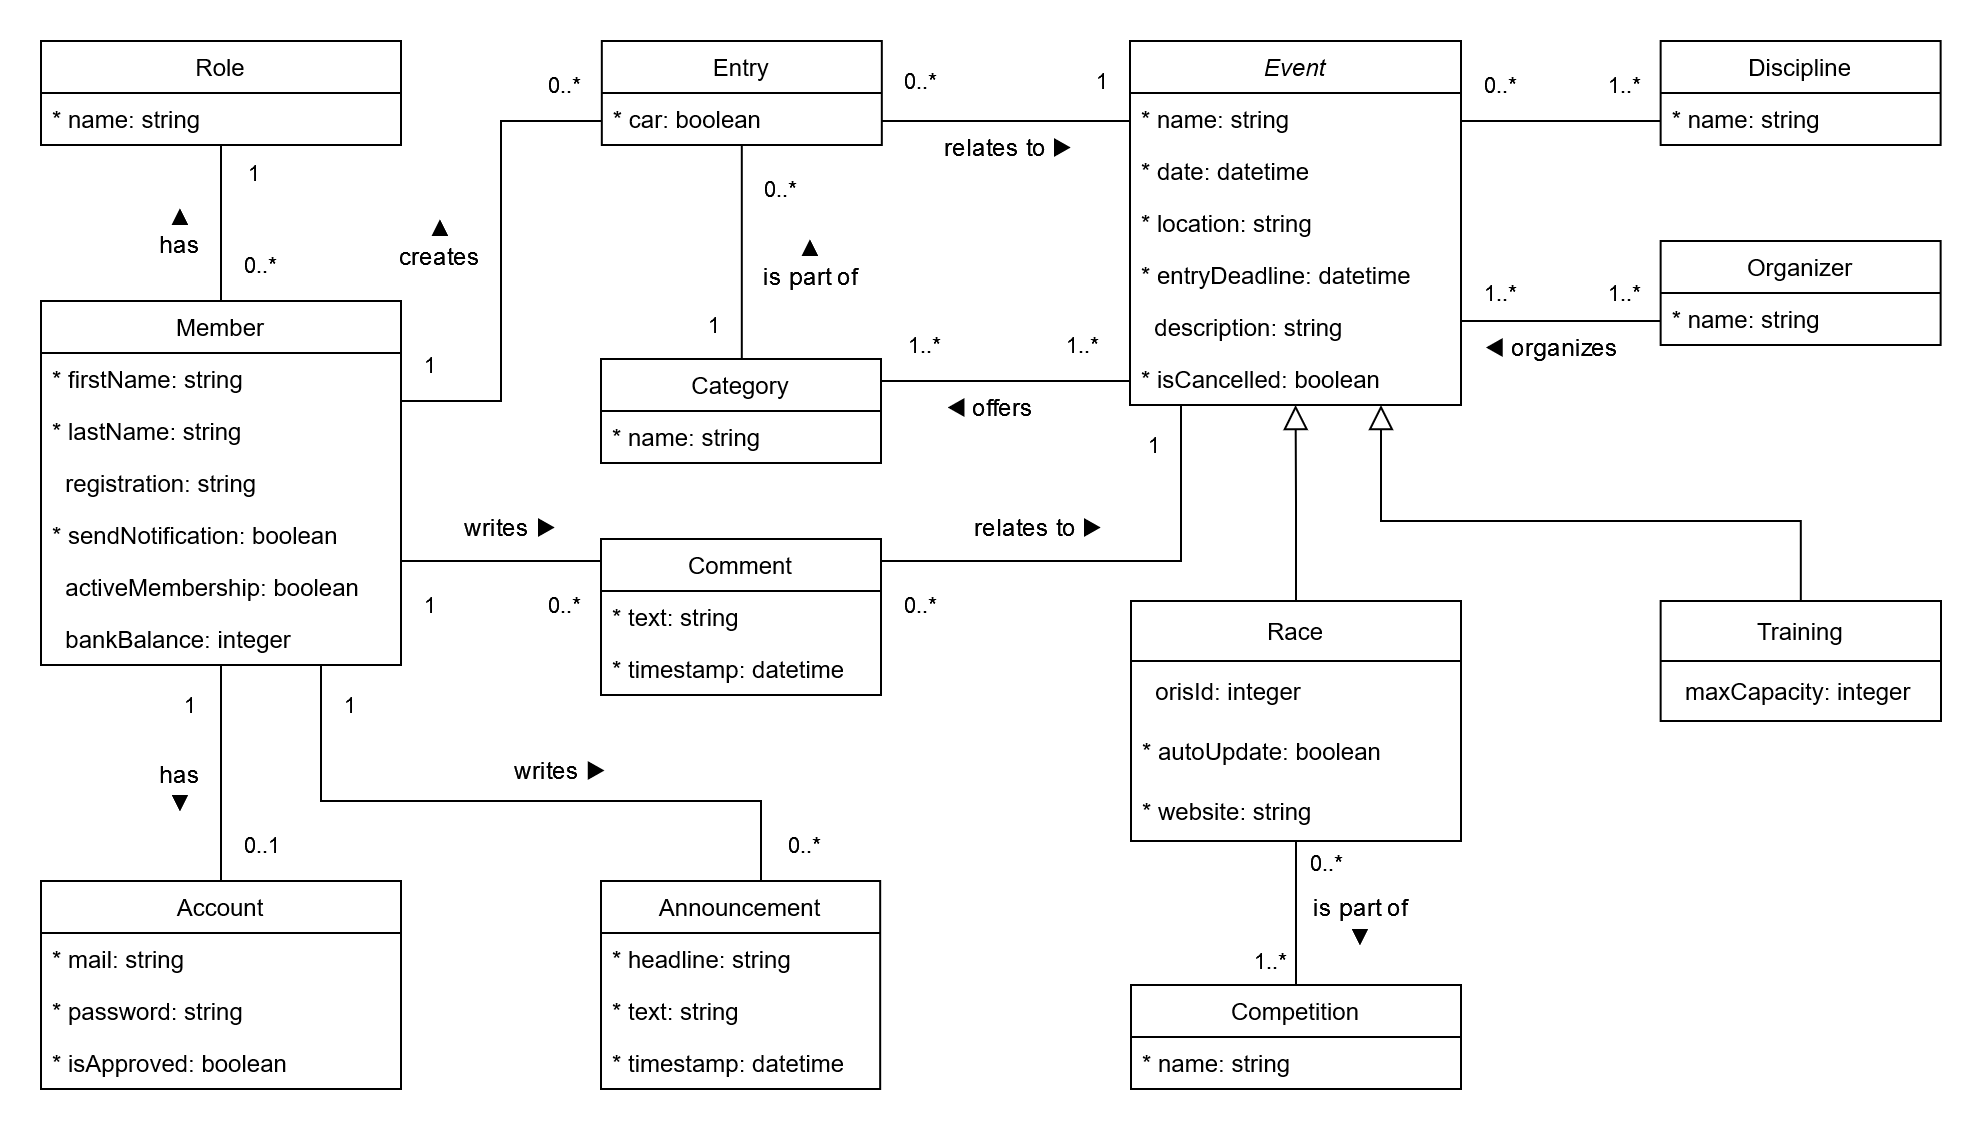
\includegraphics[width=0.95\linewidth]{images/domain-model}
	\end{figure}
\end{landscape}

\section{Doménový model}
V předchozí podkapitole byla představena MVC architektura a byly popsány její vrstvy. Tato podkapitola se zaměřuje na vrstvu modelů a bude v ní podrobněji popsáno s jakými daty bude nová aplikace pracovat. Ke znázornění modelů, jejich vlastností a vazeb mezi nimi je využit doménový model, který je vidět na obrázku \ref{figure:domain-model}. Doménový model obsahuje u každé třídy (entity) všechny vlastnosti, které se u ní plánují evidovat. Povinné vlastnosti entit jsou označeny symbolem $ \star $.

\begin{landscape}
	\begin{figure}[h]
		\caption{Doménový model}
		\label{figure:domain-model}
		\centering
		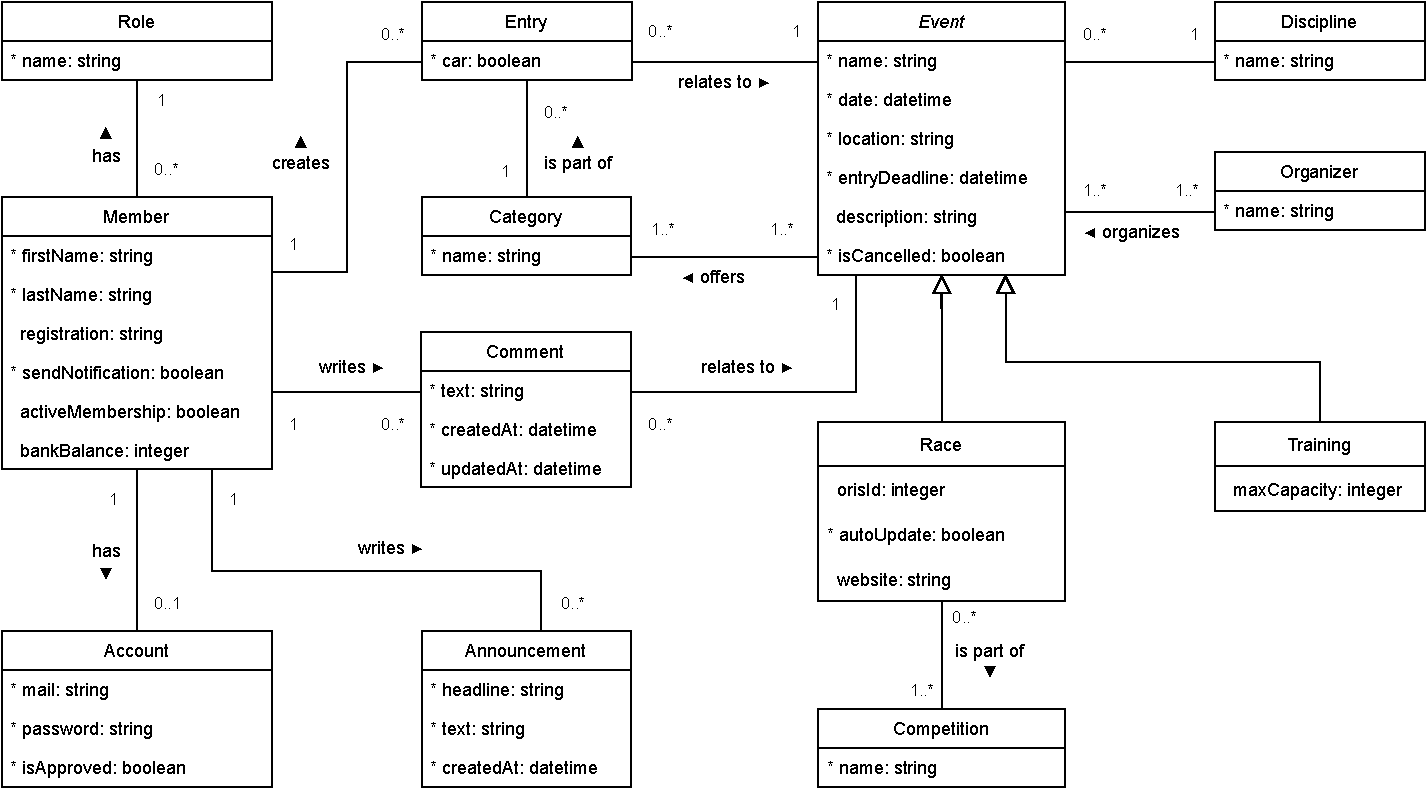
\includegraphics[width=0.9\linewidth]{images/domain-model.pdf}
	\end{figure}
\end{landscape}

\section{Technologie}
Další důležité rozhodnutí se při návrhu webové aplikace týká zvoleného programovacího jazyka, neboť je možné vybírat z mnoha možností a každý jazyk má své specifické vlastnosti. Dle W3Techs převládá mezi stránkami, u nichž je znám programovací jazyk na~straně serveru, již minimálně od roku 2011 programovací jazyk PHP. Z dostupných dat k 1. dubnu 2022 používá PHP více než 77~\% webových stránek. Mezi další využívané jazyky se následně řadí ASP.NET (7,8 \%), Ruby (6 \%) a Java (3,9 \%). \cite{php_w3techs} S ohledem na nefunkční požadavek \ref{n:technologies}, který vyžaduje vytvoření aplikace v programovacím jazyku PHP, bude pro~vývoj využit právě tento jazyk.

\subsection{PHP}
 PHP je skriptovací programátorský jazyk, který je určen především pro~vývoj webových aplikací. Nejčastěji je PHP kód spouštěn na~webovém serveru na~základě požadavku od~klienta, kterým může být například webový prohlížeč. Po~vykonání kódu je výsledek zaslán zpět klientovi. \cite{php_intro_1, php_intro_2} Nejnovější stabilní verze PHP (ke~dni 5.~2.~2022) je verze 8.1 \cite{php_version}, avšak pro~vývoj této aplikace bude z~důvodů kompatibility využita verze 8.0.
 
 Podobně jako v jiných programovacích jazycích, tak i pro jazyk PHP byla vytvořena celá řada frameworků a knihoven, které by měly usnadnit vytváření nových aplikací. Dle průzkumu za rok 2021 se mezi nejpoužívanější PHP frameworky řadí Laravel a Symfony \cite{php_jetbrains}.
 
\subsection{Symfony}
Symfony se řadí mezi nejstarší PHP frameworky, neboť se prvního vydání dočkalo již v roce 2005 \cite{symfony_legacy}. Od té doby se však neustále vyvíjí a v roce 2021 se dle průzkumu od JetBrains jednalo po Laravelu o druhý nejpoužívanější PHP framework \cite{php_jetbrains}. Symfony však není pouze samotný framework, ale je to sada znovupoužitelných komponent. To dokazuje i skutečnost, že Laravel a mnoho dalších projektů některé Symfony komponenty využívá. Mezi takové projekty se například řadí známé systémy pro správu obsahu (CMS) Drupal a Joomla! nebo řešení pro~internetové obchody PrestaShop. \cite{symfony_projects}

Pokud bychom porovnávali Laravel a Symfony, tak zjistíme, že to jsou v základu podobné frameworky a liší se spíše v drobnostech. Oba jsou založeny na MVC architektuře, v obou jsou k dispozici nástroje pro objektově relační mapování, šablonovací procesory a podobně. Zásadnější rozdíly bychom například mohli nalézt v možnostech konfigurace. Symfony v porovnání s Laravelem umožňuje pokročilejší nastavení, díky čemuž může být však obtížnější na naučení a vývoj aplikace většinou zabere i více času. U větších projektů však tyto důsledky ustupují do pozadí a vyvíjená aplikace může být přizpůsobena přesně dne potřeb cílových skupin. \cite{symfony_laravel_comparison}

Jedním z důvodů, proč jsem si pro implementaci této aplikace vybral Symfony, je skutečnost, že Laravel využívá „magii“ (například magickou metodu \mintinline{php}|__get()| pro přístup k atributům), která stěžuje statickou analýzu kódu \cite{larastan}. Dalším faktorem byla již zmíněná větší volnost při využívání Symfony frameworku a také fakt, že s používáním Symfony jsem měl již nějaké zkušenosti.

\subsection{Databáze}
Pro ukládání dat lze využít několik typů databází. V současnosti jsou stále nejpopulárnější relační databáze, které jsou občas z důvodu využívaného dotazovacího jazyka také označovány jako SQL databáze. Jejich základem jsou tabulky, které mají pevně danou strukturu. Jednotlivé řádky tabulky  představují uložené záznamy a sloupce obsahují vlastnosti daných záznamů. \cite{databases} Dnes se však kromě relačních databází můžeme setkat i s NoSQL databázemi, které například mají své uplatnění při ukládání nestrukturovaných nebo velkých dat \cite{nosql}.

Vyvíjená aplikace bude pracovat s pevně struktorovanými daty, a proto bude využita relační databáze. Vzhledem k nefunkčnímu požadavku \ref{n:technologies} se bude jednat o databázi MariaDB, která vznikla v roce 2009 jako kopie MySQL kvůli obavám jejího dalšího směřování po odkoupení společností Oracle \cite{mariadb}.

\subsection{Doctrine}
Jednou z dalších zvolených technologií pro vývoj nové aplikace je Doctrine. Výběr Doctrine je úzce spojen s výběrem frameworku, neboť Symfony přímo poskytuje možnost integrace s touto komponentou. Jedná se o sadu knihoven, které umožňují objektově relační mapování (ORM) a které nabízí objektově orientované API (a řadu dalšího) pro manipulaci s daty a se strukturou databáze \cite{doctrine_orm, doctrine_dbal}.

Při vývoji aplikací v objektově orientovaných jazycích se často využívají objekty, které nám sdružují vlastnosti předmětů podobně jako tomu je v reálném světě. Tento přístup k datům však neodpovídá tomu, jakým způsobem se data ukládají v relačních databázích. V nich je jeden konkrétní objekt reprezentován jako jeden řádek s odpovídajícím počtem sloupců. Rozdíly mezi těmito přístupy vyrovnává právě ORM, které zajišťuje automatickou konverzi dat mezi objektově orientovaným jazykem a relační databází. \cite{doctrine_orm}

Další částí Doctrine je již zmíněná abstraktní vrstva nad databází (DBAL). Díky ní nemusíme k databázi přistupovat napřímo, ale můžeme využít připravené metody, které poskytují jednotný přístup k datům a struktuře databáze nezávisle na využívaném řešení. V současnosti jsou podporovány všechny nejpoužívanější typy relačních databází zahrnující MySQL, Oracle, PostgreSQL, SQLite a Microsoft SQL Server. \cite{doctrine_dbal}

\subsection{Bootstrap}\label{bootstrap}
Poslední technologie, která bude představena v této kapitole, je Bootstrap. Jedná se svobodný a otevřený software, který usnadňuje tvorbu uživatelského rozhraní ve~webových aplikacích. Zahrnuje šablony napsané v HTML, CSS a další rozšíření implementované v jazyku JavaScript. Šablony jsou k dispozici pro všechny základní HTML elementy a umožňují jednoduše vytvářet responzivní uživatelské rozhraní. \cite{bootstrap}



\appendix\appendixinit % do not remove these two commands

\chapter{Ukázky z vytvořené aplikace}\label{appendix}

\begin{figure}[h]
    \centering
    \begin{minipage}[b]{0.48\linewidth}
        \caption{Administrace}
        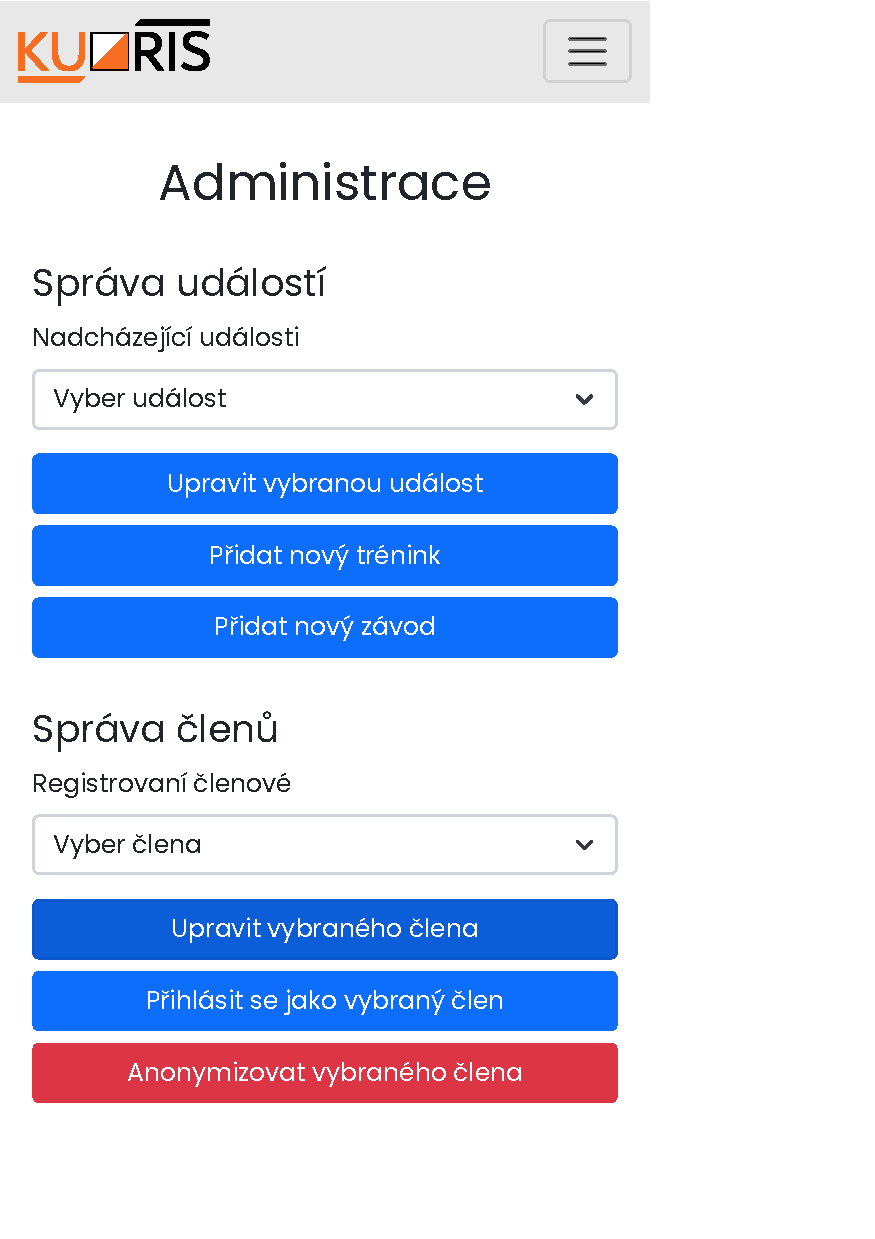
\includegraphics[width=0.99\linewidth, trim={0 2pt 0 0}, cfbox=kuorisgray 0.5pt 0pt]{images/appendix-admin.pdf}
    \end{minipage}
    \hfill
    \begin{minipage}[b]{0.48\linewidth}
        \caption{Potvrzovací dialog}
        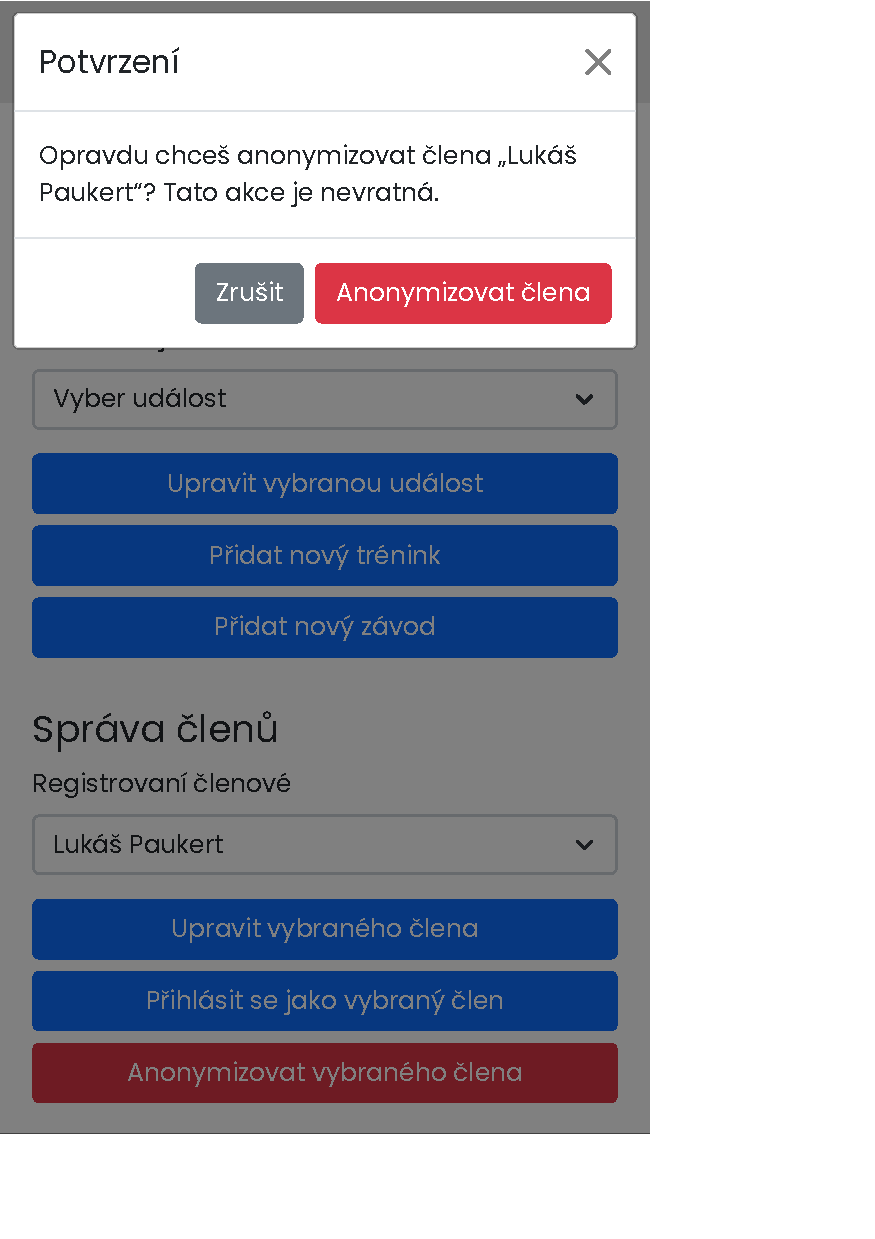
\includegraphics[width=0.99\linewidth, trim={0 1pt 0 0}]{images/appendix-admin-anonymization.pdf}
    \end{minipage}
\end{figure}

\begin{figure}[h]
    \caption{Stránka se závody}
    \centering
    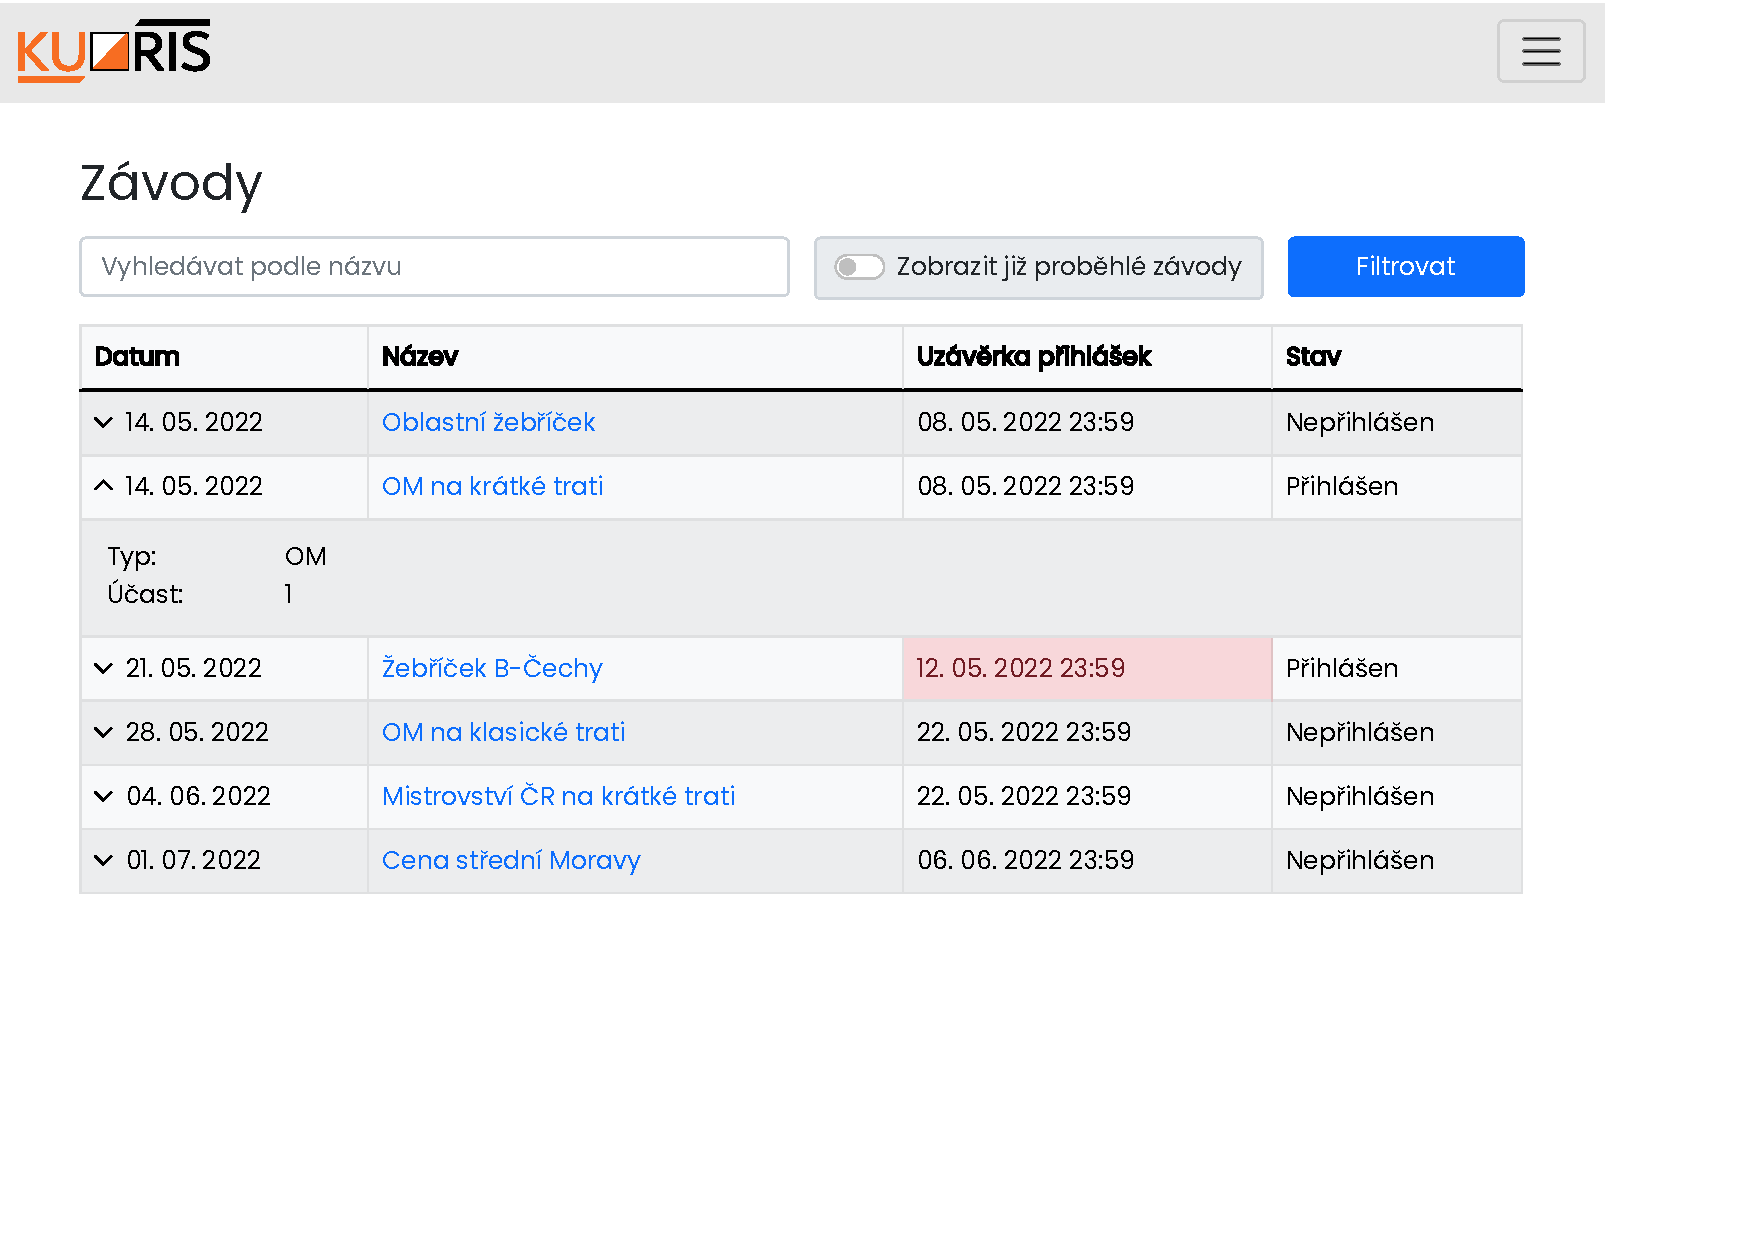
\includegraphics[width=0.995\linewidth, cfbox=kuorisgray 0.5pt 0pt]{images/appendix-races.pdf}
\end{figure}

\begin{figure}[h]
    \caption{Stránka s detailními informacemi o závodu}
    \centering
    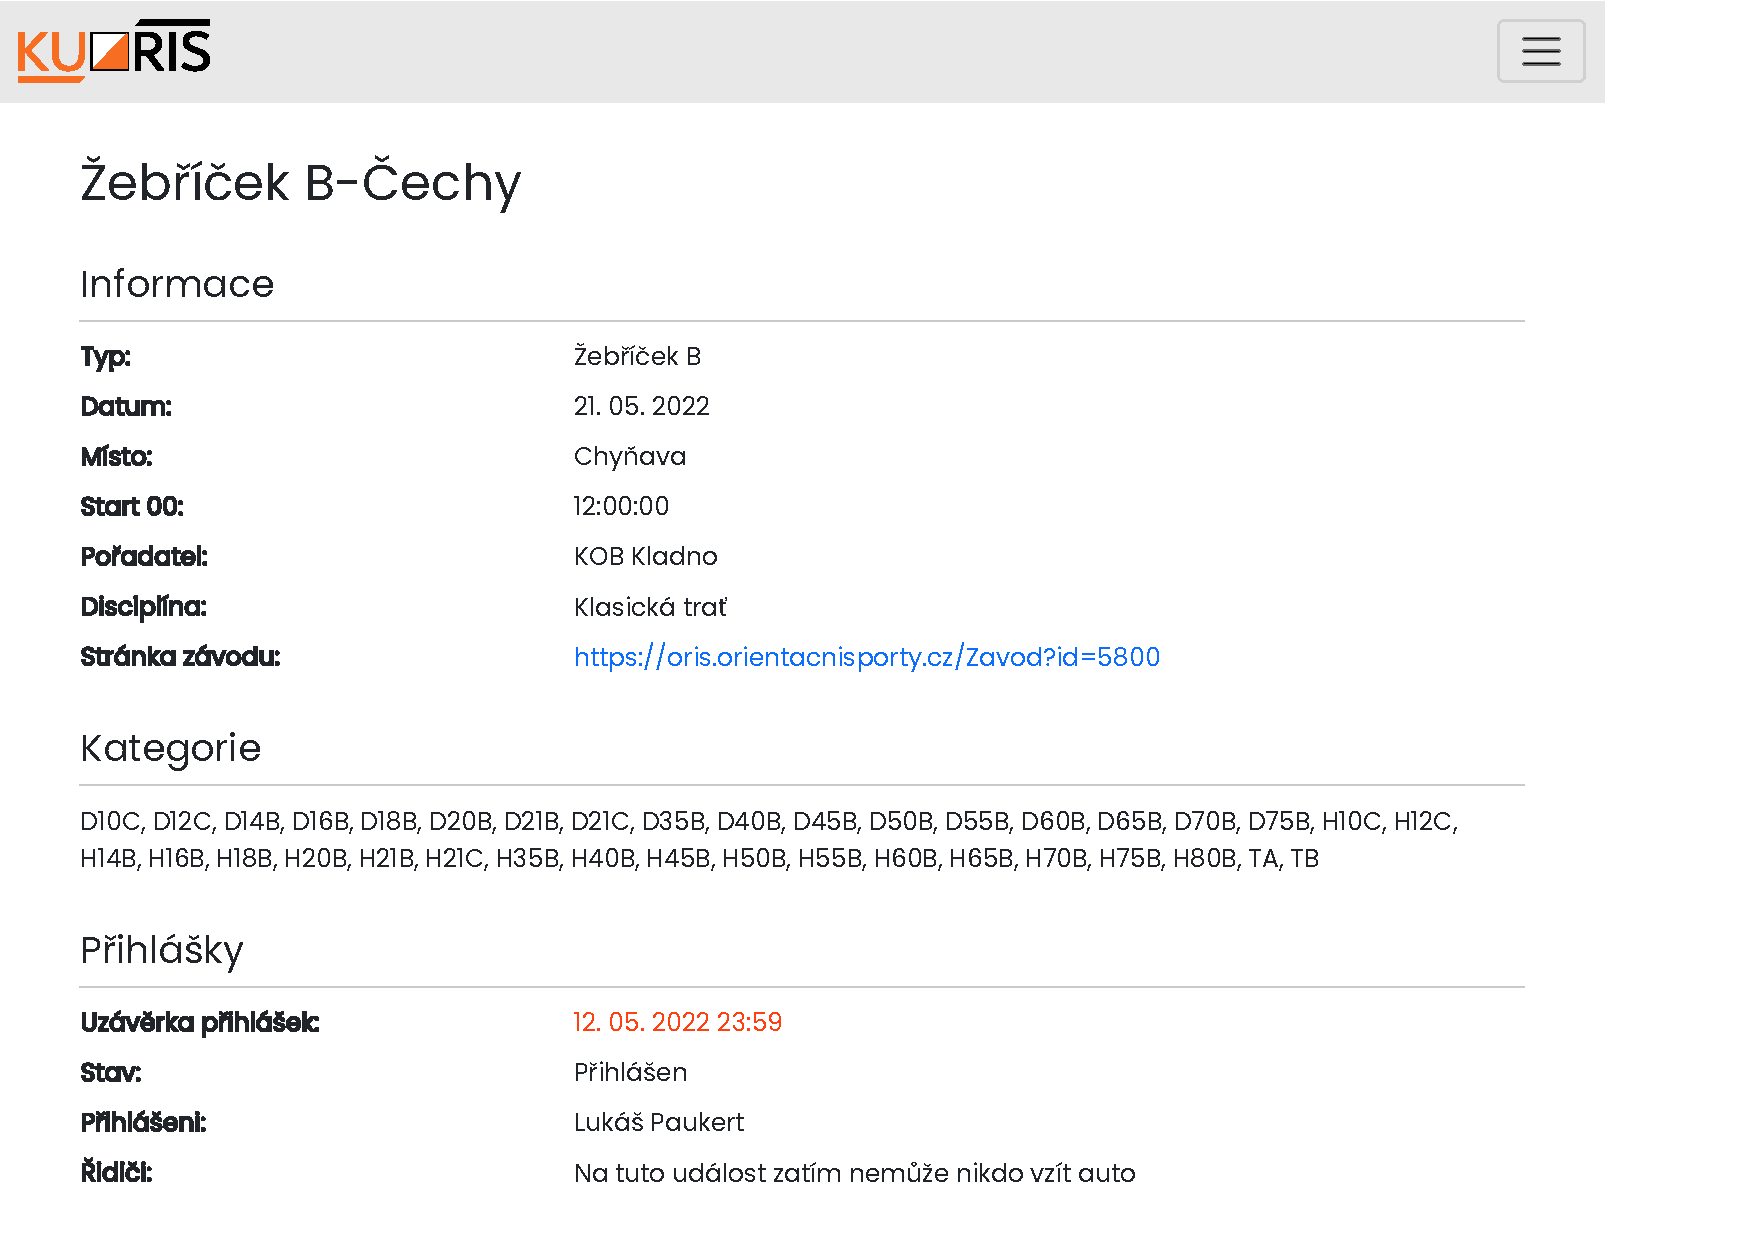
\includegraphics[width=0.995\linewidth, cfbox=kuorisgray 0.5pt 0pt]{images/appendix-detail.pdf}
\end{figure}

\begin{figure}[ht!]
    \caption{Hlavní stránka}
    \centering
    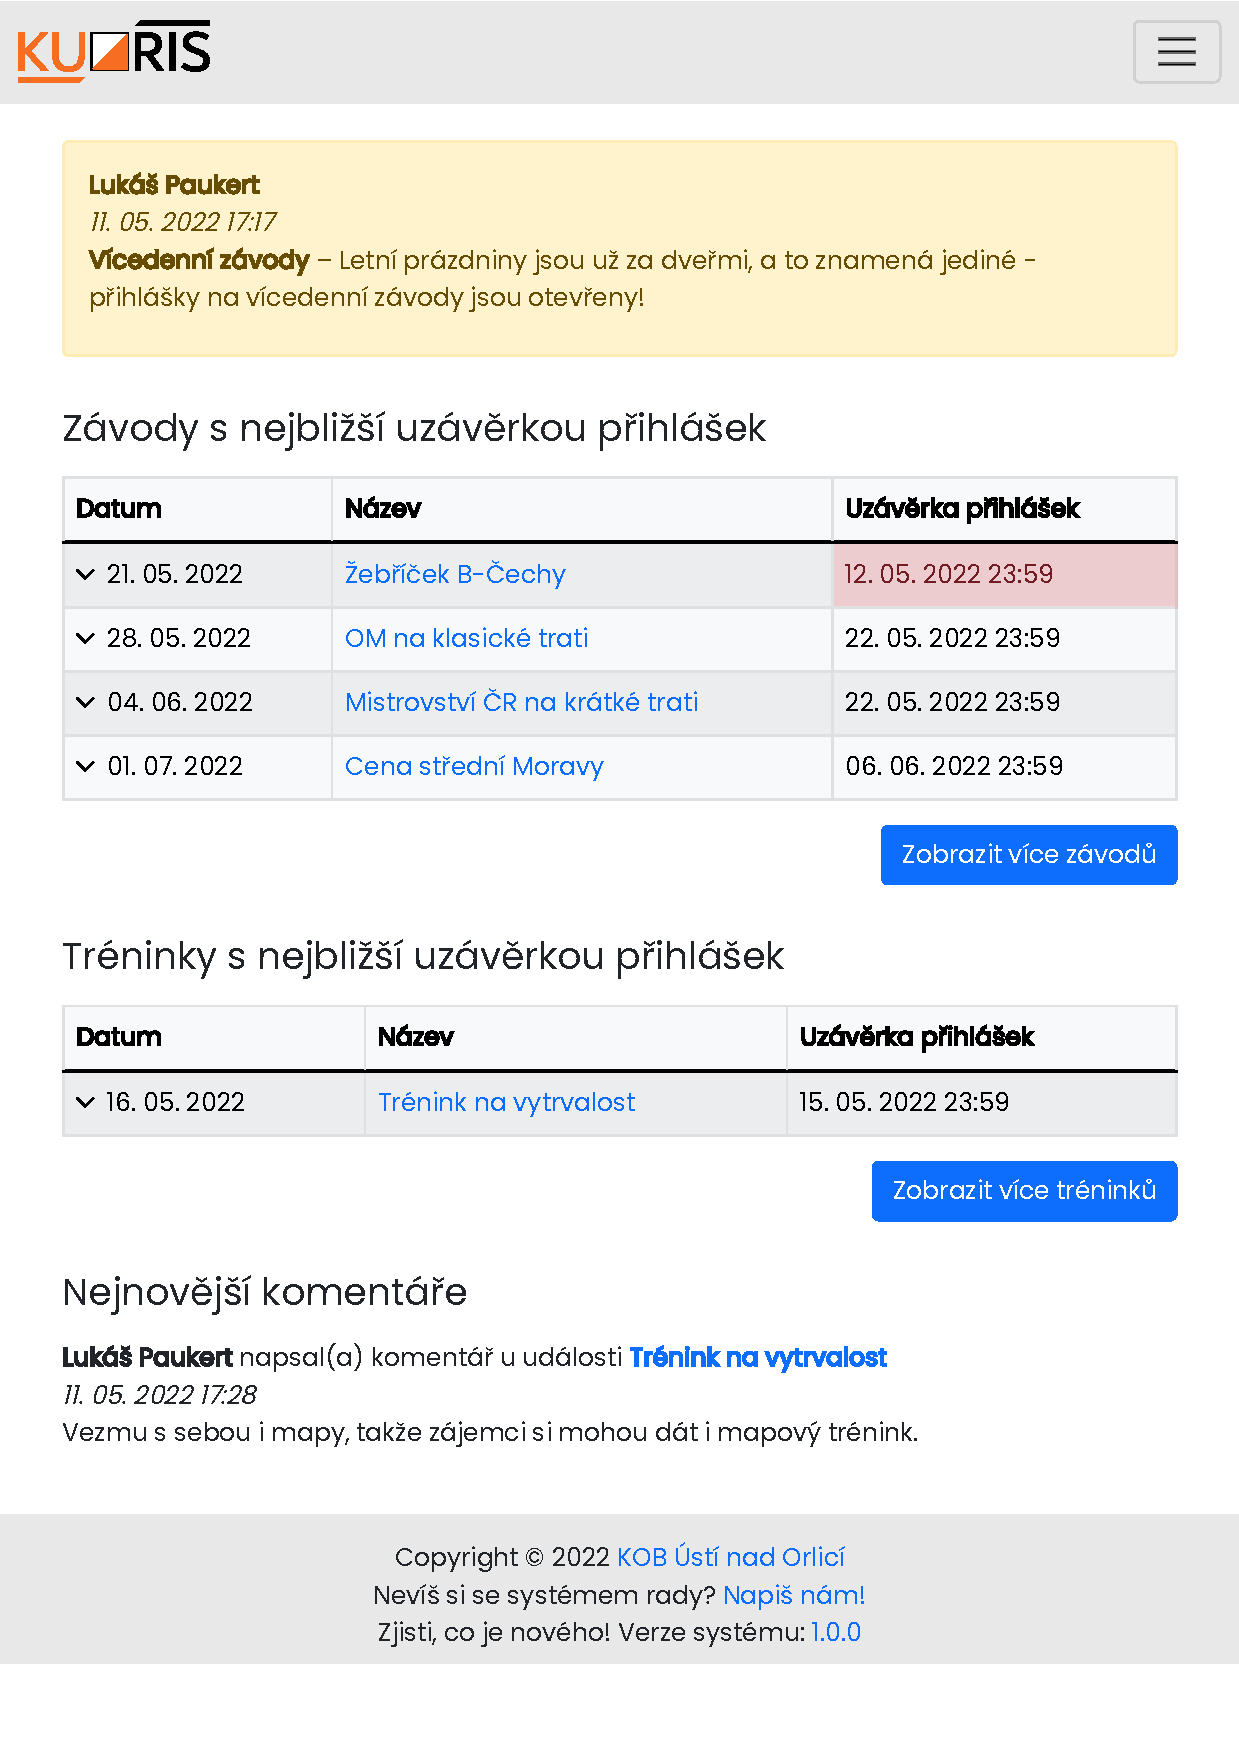
\includegraphics[width=0.995\linewidth, trim={0 1pt 0 0}, cfbox=kuorisgray 0.5pt 0pt]{images/appendix-homepage.pdf}
    \vspace{12.2mm}
\end{figure}
 % include `appendix.tex' from `parts/' subdirectory

\backmatter % do not remove this command

\printbibliography % print out the BibLaTeX-generated bibliography list

\chapter{Obsah přiloženého média}

	\dirtree{%
		.1 readme.txt\DTcomment{stručný popis obsahu média}.
		.1 doc\DTcomment{adresář s dokumentací}.
		.1 src.
		.2 impl\DTcomment{zdrojové kódy implementace}.
		.2 thesis\DTcomment{zdrojová forma práce ve formátu \LaTeX{}}.
		.1 text\DTcomment{text práce}.
		.2 BP\_Paukert.pdf\DTcomment{text práce ve formátu PDF}.
	}
 % include `medium.tex' from `parts/' subdirectory

\end{document}
